\documentclass[titlepage]{article}
\usepackage{fontspec} % For loading fonts} % For loading fonts
\usepackage{lmodern}
\usepackage[T1]{fontenc}
\usepackage[spanish,activeacute]{babel}
\usepackage{mathtools}
\usepackage{amsmath}
\usepackage{listings}
\usepackage{color} %red, green, blue, yellow, cyan, magenta, black, white
\definecolor{mygreen}{RGB}{28,172,0} % color values Red, Green, Blue
\definecolor{mylilas}{RGB}{170,55,241}
\usepackage{graphicx}
\usepackage{float}

% Datos de la portada
\title{Filtros software en el proyecto SHFD}
\date{} % para que no aparezca la fecha la dejo en blanco

\begin{document}
\maketitle
En este documento se muestra como se ha realizado el cálculo de coeficientes de la librería de filtros que se utilizan en el proyecto SHFD. Hay tres familias de filtros: filtros de primer orden, filtros de segundo orden, y filtros de orden superior. 

Este documento no tiene más ámbito que el de documentar la obtención de los coeficientes digitales de filtros de primer y segundo orden, a partir de la especificación de los parámetros que los definen. En los filtros de primer orden los parámetros serán :  la frecuencia de muestreo , y la frecuencia de corte. En los filtros de segundo orden los parámetros serán: frecuencia de muestreo, frecuencia de corte/paso y factor de calidad.

En las siguientes secciones veremos como obtener los coeficientes en filtros de primer orden, y en filtros de segundo orden.

\section{Filtros de primer orden:}
\subsection{Filtro paso bajo}
\subsubsection{Transformada de Laplace del filtro}
\begin{equation}
\label{eqn:Hs_primer_orden_paso_bajo}Hs(s)=\frac{1}{\displaystyle\frac{s}{{\omega_o}}+1}=\frac{\displaystyle\omega_o}{s+\omega_o}
\end{equation}
\quad siendo ${\omega_o}=2{\pi}fc$  y fc la frecuencia de corte del filtro. 
\subsubsection{Mapeo de polos y ceros en el plazo z}
Como se puede extraer de (\ref{eqn:Hs_primer_orden_paso_bajo}) tenemos un polo en $s=-{\omega_o}$, y por lo tanto el filtro digital tendrá un polo en $z=e^{-\omega_oT}$ 
\begin{equation}
	H(z)=K\frac{1}{z-e^{-\omega_oT}} 
\end{equation}
\subsubsection{Valor de la ganancia}
Buscamos determinar el valor de la ganancia K para obtener el mismo resultado en el filtro digital y analógico en el rango de frecuencias de los filtros. Comparamos la ganancia de ambos filtros a la misma frecuencia  
\subsubsection{Cálculo de ganancia a frecuencias bajas}
\begin{equation}
\label{eqn:lim_Hs_primer_orden_paso_bajo}\lim_{\omega \to 0}Hs(j\omega)=1
\end{equation}
\begin{equation}
\label{eqn:lim_Hz_primer_orden_paso_bajo}\lim_{\omega \to 0}H(e^{j\omega_oT})=\frac{K}{1-e^{-\omega_oT}}
\end{equation}
\quad igualando \ref{eqn:lim_Hs_primer_orden_paso_bajo} y \ref{eqn:lim_Hz_primer_orden_paso_bajo} obtenemos $K=1-e^{-\omega_oT}$ 
\subsubsection{Ecuación final en diferencias}
Sustituyendo K en la en la función de transferencia en z obtenemos 
\begin{equation}
	H(z)=\frac{1-e^{-\omega_oT}}{z-e^{-\omega_oT}}=\frac{(1-e^{-\omega_oT})z^{-1}}{1-e^{-\omega_oT}z^{-1}} 
\end{equation}
La ecuación en diferencias es:
\begin{equation}
\label{eqn:dif_primer_orden_paso_bajo}y_n=e^{-\omega_oT}y_{n-1}+(1-e^{-\omega_oT})x_{n-1}
\end{equation}
\subsubsection{Eliminación de retardo en el filtro}
Como se aprecia en (\ref{eqn:dif_primer_orden_paso_bajo}) no hacemos uso de $x_n$ sino de $x_{n-1}$, para eliminar este retardo basta con añadir un zero en el origen, veamos como queda la función de transferencia final:
\begin{equation}
	H(z)=\frac{(1-e^{-\omega_oT})z}{z-e^{-\omega_oT}}=\frac{1-e^{-\omega_oT}}{1-e^{-\omega_oT}z^{-1}} 
\end{equation}
La ecuación en diferencias final es:
\begin{equation}
y_n=e^{-\omega_oT}y_{n-1}+(1-e^{-\omega_oT})x_{n}
\end{equation}
\subsubsection{Coeficientes del filtro}
\begin{equation}
y_n=e^{-\omega_oT}y_{n-1}+(1-e^{-\omega_oT})x_{n} => a_0y_{n}=a_1y_{n-1}+b_0x_n
\end{equation}
siguiendo la estructura estándar de filtros digitales:
\begin{equation}
y[n]=(b_0x[n]+b_1x[n-1]+ ....)-(a_1y[n-1] + a_2y[n-2] + .....)  
\end{equation}
los coeficientes finales que obtenemos son:
\begin{equation}
a_0=1;
a_1=e^{-\omega_oT};
b_0=1-e^{-\omega_oT}
\end{equation}
\subsubsection{Código de Matlab}
\lstset{language=Matlab,%
	basicstyle=\scriptsize,
    breaklines=true,%
    morekeywords={matlab2tikz},
    keywordstyle=\color{blue},%
    morekeywords=[2]{1}, keywordstyle=[2]{\color{black}},
    identifierstyle=\color{black},%
    stringstyle=\color{mylilas},
    commentstyle=\color{mygreen},%
    showstringspaces=false,%without this there will be a symbol in the places where there is a space
%    numbers=left,%
    numberstyle={\tiny \color{black}},% size of the numbers
    numbersep=9pt, % this defines how far the numbers are from the text
    emph=[1]{for,end,break},emphstyle=[1]\color{red}, %some words to emphasise
    %emph=[2]{word1,word2}, emphstyle=[2]{style},    
}
\lstinputlisting{filtro_paso_bajo_minimo_retardo.m}
\subsubsection{Respuesta en frecuencia del filtro}
En la siguiente gráfica \ref{fig:filtro_paso_bajo_minimo_retardo} se muestra la respuesta del filtro de paso bajo digital, y la misma respuesta pero con fase mínima (eliminando el retardo del filtro). Como se puede observar la utilización del zero para eliminar el retardo, implica no tener la misma respuesta en fase.
\begin{figure}[H]
  \centering
	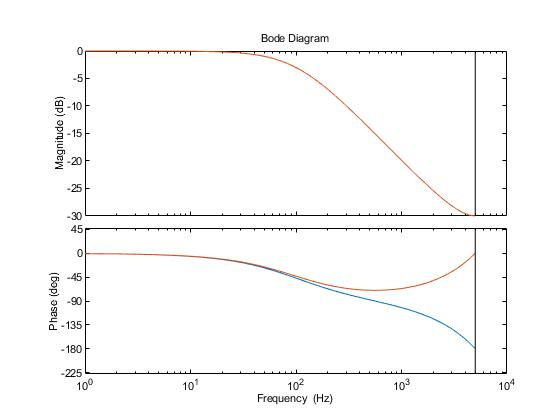
\includegraphics[scale=0.5]{filtro_paso_bajo_minimo_retardo}
  \caption{Respuesta en frecuencia del filtro paso bajo con retardo mínimo}
  \label{fig:filtro_paso_bajo_minimo_retardo}
\end{figure}
\subsubsection{Implementación}
Al método software que se encarga de ejecutar este filtrado , se le deberán pasar los siguientes parámetros:
\begin{enumerate}
\item Frecuencia de muestro 
\item Frecuencia de corte
\end{enumerate}
Con estos parámetros el método software se encargará de extraer los coeficientes como se ha visto en los puntos anteriores y, realizar el filtrado de la muestra de entrada.





\subsection{Filtro paso alto}
\subsubsection{Transformada de Laplace del filtro}
\begin{equation}
\label{eqn:tfs_filtro_paso_alto_primer_orden} Hs(s)=\frac{\displaystyle\frac{s}{\omega_o}}{\displaystyle\frac{s}{{\omega_o}}+1} = \frac{s}{s+\omega_o}
\end{equation}
\quad siendo ${\omega_o}=2{\pi}fc$ ;fc es la frecuencia de corte del filtro 
\subsubsection{Mapeo de polos y ceros en el plazo z}
Como se puede extraer de \ref{eqn:tfs_filtro_paso_alto_primer_orden} tenemos:

\begin{enumerate}
\item Un polo en $s=-{\omega_o}$, y por lo tanto el filtro digital tendrá un polo en $z=e^{-\omega_oT}$ 
\item Un cero en el origen $s=0$, y por lo tanto el filtro digital tendrá un cero en $z=1"$
	\begin{equation}
		H(z)=K\frac{z-1}{z-e^{-\omega_oT}} 
	\end{equation}
\end{enumerate}

\subsubsection{Valor de la ganancia}
Buscamos determinar el valor de la ganancia K para obtener el mismo resultado en el filtro digital y analógico en el rango de frecuencias de los filtros. Comparamos la ganancia de ambos filtros a la misma frecuencia.

\subsubsection{Cálculo de ganancia a frecuencias bajas}
\begin{equation}
\label{eq:lim_Hs_primer_orden_paso_alto}\lim_{\omega \to \omega_o}Hs(j\omega)=10^\frac{-3}{20}(3db)
\end{equation}
\begin{equation}
\label{eq:lim_Hz_primer_orden_paso_alto}\lim_{\omega \to \omega_o}H(e^{j\omega_oT})=K\frac{e^{j\omega_oT} -1}{e^{j\omega_oT}-e^{-\omega_oT}}
\end{equation}
\quad igualando \ref{eq:lim_Hs_primer_orden_paso_alto} y \ref{eq:lim_Hz_primer_orden_paso_alto} obtenemos el valor de la ganancia K.


\subsubsection{Ecuación final en diferencias}
\begin{equation}
		H(z)=K\frac{z-1}{z-e^{-\omega_oT}} = K\frac{1 - z^{-1}}{1-e^{-\omega_oT}z^{-1}}
\end{equation}
La ecuación en diferencias es:
\begin{equation}
\label{eqn:dif_primer_orden_paso_alto}y_n=e^{-\omega_oT}y_{n-1}+ Kx_{n} - Ke^{-\omega_oT}x_{n-1}
\end{equation}
\subsubsection{Coeficientes del filtro}
\begin{equation}
y_n=e^{-\omega_oT}y_{n-1}+(x_{n}-e^{-\omega_oT})x_{n-1} => a_0y_{n}=a_1y_{n-1}+b_0x_n + b1x{n-1}
\end{equation}
siguiendo la estructura estándar de filtros digitales:
\begin{equation}
y[n]=(b_0x[n]+b_1x[n-1]+ ....)-(a_1y[n-1] + a_2y[n-2] + .....)  
\end{equation}
los coeficientes finales que obtenemos son:
\begin{equation}
a_0=1;
a_1=e^{-\omega_oT};
b_0=1;
b_1=-1
\end{equation}

\subsubsection{Código de Matlab}
\lstset{language=Matlab,%
	basicstyle=\scriptsize,
    breaklines=true,%
    morekeywords={matlab2tikz},
    keywordstyle=\color{blue},%
    morekeywords=[2]{1}, keywordstyle=[2]{\color{black}},
    identifierstyle=\color{black},%
    stringstyle=\color{mylilas},
    commentstyle=\color{mygreen},%
    showstringspaces=false,%without this there will be a symbol in the places where there is a space
%    numbers=left,%
    numberstyle={\tiny \color{black}},% size of the numbers
    numbersep=9pt, % this defines how far the numbers are from the text
    emph=[1]{for,end,break},emphstyle=[1]\color{red}, %some words to emphasise
    %emph=[2]{word1,word2}, emphstyle=[2]{style},    
}
\lstinputlisting{filtro_paso_alto_primer_orden.m}

\subsubsection{Respuesta en frecuencia del filtro}
En la siguiente gráfica \ref{fig:filtro_paso_alto_primer_orden} se muestra la respuesta del filtro de paso alto digital.
\begin{figure}[H]
  \centering
	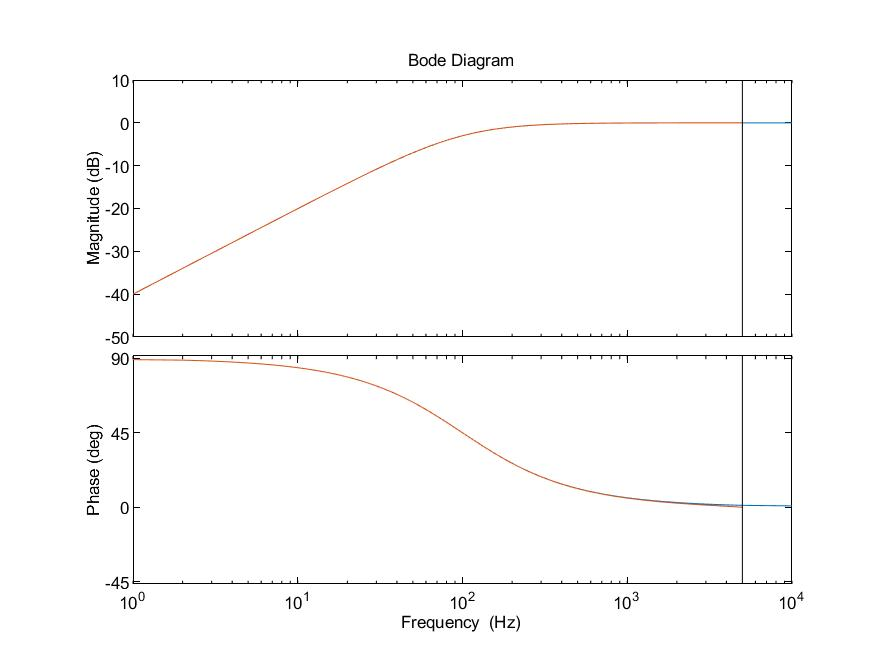
\includegraphics[scale=0.4]{filtro_paso_alto_primer_orden}
  \caption{Respuesta en frecuencia del filtro paso alto}
  \label{fig:filtro_paso_alto_primer_orden}
\end{figure}
\subsubsection{Implementación}
Al método software que se encarga de ejecutar este filtrado , se le deberán pasar los siguientes parámetros:
\begin{enumerate}
\item Frecuencia de muestro 
\item Frecuencia de corte
\end{enumerate}
Con estos parámetros el método software se encargará de extraer los coeficientes como se ha visto en los puntos anteriores y, realizar el filtrado de la muestra de entrada.


\section{Filtros de segundo orden:}
En las siguientes secciones se muestran los filtros de segundo orden implementados:
\subsection{Filtro paso bajo}
\subsubsection{Transformada de Laplace del filtro}
\begin{equation}
Hs(s)=\frac{1}{\displaystyle{(\frac{s}{\omega_0}})^2+2\zeta\frac{s}{\omega_0}+1}
\end{equation}
sabiendo que el factor de calidad del filtro paso bajo es $Q=\displaystyle\frac{1}{2\zeta}$ y, $\omega_0=2{\pi}fc$ siendo fc la frecuencia de corte.
\subsubsection{Mapeo de polos y ceros en el plazo z}
La función de transferencia anterior se puede expresar como el producto de dos polos complejos conjugados y una ganancia.  
\begin{equation}
Hs(s)=\frac{K}{\displaystyle(s+p)(s+\hat{p})}
\end{equation}
donde  $p=-\sigma+j\omega$ y $\hat{p}=-\sigma-j\omega$.
Mapeando (13) en el plano z obtenemos
\begin{equation}
H(z)=\frac{K}{\displaystyle(z-e^{(-\sigma+j\omega)T})(z-e^{(-\sigma-j\omega)T})}
\end{equation}

desarrollando la multiplicación del dividendo de (14) obtenemos
\begin{equation}
z^2+z[e^{(-\sigma+j\omega)T}+e^{(-\sigma-j\omega)T}]+e^{-(2\sigma)T}  
\end{equation}
%\begin{equation}
%z^2+ze^{-T\sigma}[\cos{({\omega}T)}+\cos{(-{\omega}T)}+j%%\sin{({\omega}T)}
%+j\sin{(-{\omega}T)}]+e^{-(2{\sigma}T)} 
%\end{equation}
%\begin{equation}
%z^2-ze^{{-\sigma}T}[\cos{({\omega}T)} + \cos{(-{\omega}T)}]%+e^{-2{\sigma}T}
%\end{equation}


De la ecuación (12) podemos obtener los valores de $\sigma$ y $\omega$
\begin{equation}
\sigma=-(\omega_0/Q)/2
\end{equation}

\begin{equation}
\omega=\frac{\sqrt{(\frac{\displaystyle\omega_o}{Q})^2-4\omega_o^2}}{2}
\end{equation}

\subsubsection{Valor de la ganancia}
Se busca determinar el valor de la ganancia K para obtener el mismo resultado en el filtro digital y en el filtro analógico. Para ello se iguala la ganancia de ambos filtros a la misma frecuencia.
\subsubsection{Cálculo de ganancia a frecuencias bajas}
Para obtener la ganancia K, se realiza el límite de las funciones H(s) y la anterior H(z) en la banda de paso, para un filtro paso bajo se ha decidido que la frecuencia de comparación de $\omega_0$ sea 0 rad/s. 
\begin{equation}
\label{eq:lim_Hs_paso_bajo}\lim_{\omega \to 0}Hs(j\omega)=1
\end{equation}
\begin{equation}
\label{eq:lim_Hz_paso_bajo}\lim_{\omega \to 0}H(e^{j\omega})=\frac{K}{a_2+a_1+a_0}
\end{equation}
\quad igualando \ref{eq:lim_Hs_paso_bajo} y \ref{eq:lim_Hz_paso_bajo} obtenemos $K=a_2+a_1+a_0$ 
\subsubsection{Ecuación final en diferencias}
\begin{equation}
H(z)=\frac{K}{z^2-z(e^{(-\sigma+j\omega)T}+e^{(-\sigma-j\omega)T}) + e^{-2{\sigma}T}}
\end{equation}
La ecuación en diferencias es:
\begin{equation}
a_0y_n=Kx_{n-2}-[a_1y_{n-1} + a_2y_{n-2}]
\end{equation}
\subsubsection{Coeficientes del filtro}
Siguiendo la estructura estándar de filtros digitales:
\begin{equation}
a_0y[n]=(b_0x[n]+b_1x[n-1]+ ....)-(a_1y[n-1] + a_2y[n-2] + .....)  
\end{equation}
los coeficientes finales que obtenemos son:
\begin{equation}
a_0=1
\end{equation}

\begin{equation}
a_1=-(e^{(-\sigma+j\omega)T}+e^{(-\sigma-j\omega)T})
\end{equation}

%\begin{equation}
%a_1=-e^{{-\sigma}T}[\cos{({\omega}T)} + \cos{(-{\omega}T)}]
%\end{equation}

\begin{equation}
a_2=e^{-2{\sigma}T}
\end{equation}

\subsubsection{Código de Matlab}
\lstset{language=Matlab,%
    %basicstyle=\color{red},
    basicstyle=\scriptsize,
    breaklines=true,%
    morekeywords={matlab2tikz},
    keywordstyle=\color{blue},%
    morekeywords=[2]{1}, keywordstyle=[2]{\color{black}},
    identifierstyle=\color{black},%
    stringstyle=\color{mylilas},
    commentstyle=\color{mygreen},%
    showstringspaces=false,%without this there will be a symbol in the places where there is a space
%    numbers=left,%
    numberstyle={\tiny \color{black}},% size of the numbers
    numbersep=9pt, % this defines how far the numbers are from the text
    emph=[1]{for,end,break},emphstyle=[1]\color{red}, %some words to emphasise
    %emph=[2]{word1,word2}, emphstyle=[2]{style},    
}
\lstinputlisting{lowpassdiscrete.m}
\subsubsection{Respuesta en frecuencia del filtro}
En la siguiente gráfica se muestra \ref{fig:lowpassdiscrete} la respuesta del filtro de segundo orden paso bajo, y su respuesta digital con la aproximación de mapeo de polos que hemos realizado. 
\begin{figure}[H]
  \centering
	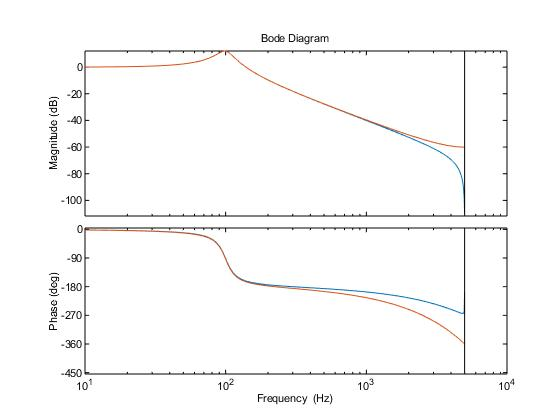
\includegraphics[scale=0.5]{lowpassdiscrete}
  \caption{Respuesta en frecuencia del filtro paso bajo de segundo orden}
  \label{fig:lowpassdiscrete}
\end{figure}

\subsubsection{Implementación}
Al método software que se encarga de ejecutar este filtrado , se le deberán pasar los siguientes parámetros:
\begin{enumerate}
\item Frecuencia de muestro 
\item Frecuencia de corte
\item Factor de calidad
\end{enumerate}
Con estos parámetros el método software se encargará de extraer los coeficientes como se ha visto en los puntos anteriores y, realizar el filtrado de la muestra de entrada.



\subsection{Filtro paso banda}
\subsubsection{Transformada de Laplace del filtro}
\begin{equation}
Hs(s)=\frac{\displaystyle\frac{2\zeta}{\omega_0}s}{\displaystyle{(\frac{s}{\omega_0}})^2+2\zeta\frac{s}{\omega_0}+1}
\end{equation}
\subsubsection{Mapeo de polos y ceros en el plazo z}
La función de transferencia anterior se puede expresar como el producto de dos polos complejos conjugados, un cero en el origen y una ganancia.  
\begin{equation}
Hs(s)=\frac{Ks}{\displaystyle(s+p)(s+\hat{p})}
\end{equation}
donde  $p=-\sigma+j\omega$ y $\hat{p}=-\sigma-j\omega$.
Mapeando (27) en el plano z obtenemos
\begin{equation}
H(z)=\frac{K(z-1)}{\displaystyle(z-e^{(-\sigma+j\omega)T})(z-e^{(-\sigma-j\omega)T})}
\end{equation}
esta función de transferencia también la podemos expresar como :
\begin{equation}
H(z)=\frac{K(z-1)}{z^2-z(e^{(-\sigma+j\omega)T}+e^{(-\sigma-j\omega)T}) + e^{-2{\sigma}T}}
\end{equation}

\subsubsection{Valor de la ganancia}
Buscamos determinar el valor de la ganancia K para obtener el mismo resultado en el filtro digital y analógico en el rango de frecuencias de los filtros. Comparamos la ganancia de ambos filtros a la misma frecuencia 
\subsubsection{Cálculo de ganancia a frecuencias de paso}
Ahora realizamos el límite de la funciones H(s) y la anterior H(z) en la frecuencia de paso $\omega_0$, al igualar el resultado de ambas f.d.t podemos obtener la ganancia K necesaria para obtener la misma respuesta en el dominio continuo y en el dominio discreto.
\begin{equation}
\label{eq:lim_Hs_paso_banda}\lim_{\omega \to \omega_0}Hs(j\omega)=1
\end{equation}
%num_in_wn=exp(i*wn*Ts)-1
%den_in_wn=a0*exp(i*2*wn*Ts)+a_1*exp(i*wn*Ts)+a_2
%gain_in_wn=1;
%K1=gain_in_wn/abs(num_in_wn/den_in_wn);
\begin{equation}
\label{eq:lim_Hz_paso_banda}\lim_{\omega \to \omega_0}H(e^{j\omega})=K\frac{e^{j\omega_0T}-1}{a_0e^{j2\omega_0T}+a_1e^{j\omega_0T}+a_2}
\end{equation}
Igualando \ref{eq:lim_Hs_paso_banda} y \ref{eq:lim_Hz_paso_banda} obtendremos el valor final de K.
\subsubsection{Ecuación final en diferencias}
\begin{equation}
H(z)=\frac{K(z-1)}{z^2-z(e^{(-\sigma+j\omega)T}+e^{(-\sigma-j\omega)T}) + e^{-2{\sigma}T}}
\end{equation}
La ecuación en diferencias es:
\begin{equation}
a_0y_n=K(x_{n-2}+x_{n-1})-[a_1y_{n-1} + a_2y_{n-2}]
\end{equation}

\subsubsection{Coeficientes del filtro}
Siguiendo la estructura estándar de filtros digitales:
\begin{equation}
a_0y[n]=(b_0x[n]+b_1x[n-1]+ ....)-(a_1y[n-1] + a_2y[n-2] + .....)  
\end{equation}
los coeficientes finales que obtenemos son:
\begin{equation}
a_0=1
\end{equation}
\begin{equation}
a_1=-(e^{(-\sigma+j\omega)T}+e^{(-\sigma-j\omega)T})
\end{equation}
\begin{equation}
a_2=e^{-2{\sigma}T}
\end{equation}

\subsubsection{Código de Matlab}
\lstset{language=Matlab,%
    basicstyle=\scriptsize,
    breaklines=true,%
    morekeywords={matlab2tikz},
    keywordstyle=\color{blue},%
    morekeywords=[2]{1}, keywordstyle=[2]{\color{black}},
    identifierstyle=\color{black},%
    stringstyle=\color{mylilas},
    commentstyle=\color{mygreen},%
    showstringspaces=false,%without this there will be a symbol in the places where there is a space
%    numbers=left,%
    numberstyle={\tiny \color{black}},% size of the numbers
    numbersep=9pt, % this defines how far the numbers are from the text
    emph=[1]{for,end,break},emphstyle=[1]\color{red}, %some words to emphasise
    %emph=[2]{word1,word2}, emphstyle=[2]{style},    
}
\lstinputlisting{bandpassdiscrete.m}
\subsubsection{Respuesta en frecuencia del filtro}
En la siguiente gráfica se muestra \ref{fig:bandpassdiscrete} la respuesta del filtro de segundo orden paso banda, y su respuesta digital con la aproximación de mapeo de polos/ceros que hemos realizado. 
\begin{figure}[H]
  \centering
	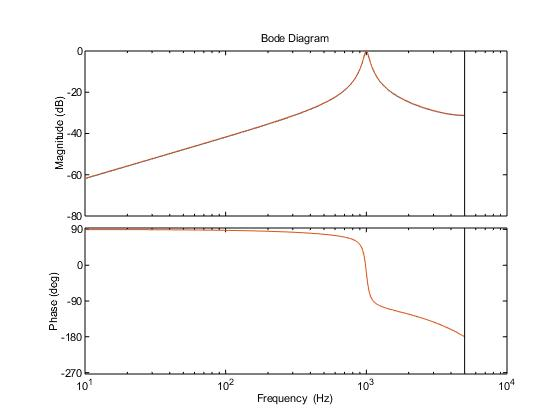
\includegraphics[scale=0.5]{bandpassdiscrete}
  \caption{Respuesta en frecuencia del filtro paso banda de segundo orden}
  \label{fig:bandpassdiscrete}
\end{figure}

\subsubsection{Implementación}
Al método software que se encarga de ejecutar este filtrado , se le deberán pasar los siguientes parámetros:
\begin{enumerate}
\item Frecuencia de muestro 
\item Frecuencia de corte
\item Factor de calidad
\end{enumerate}
Con estos parámetros el método software se encargará de extraer los coeficientes como se ha visto en los puntos anteriores y, realizar el filtrado de la muestra de entrada.









\subsection{Filtro paso alto}
\subsubsection{Transformada de Laplace del filtro}
\begin{equation}
Hs(s)=\frac{(\displaystyle\frac{s}{\omega_0})^2}{\displaystyle{(\frac{s}{\omega_0}})^2+2\zeta\frac{s}{\omega_0}+1}
\end{equation}
\subsubsection{Mapeo de polos y ceros en el plazo z}
La función de transferencia anterior se puede expresar como el producto de dos polos complejos conjugados, un cero doble en el origen, y una ganancia.
\begin{equation}
\label{eq:Hs_paso_alto}Hs(s)=\frac{Ks^2}{\displaystyle(s+p)(s+\hat{p})}
\end{equation}
Mapeando \ref{eq:Hs_paso_alto} en el plano z obtenemos
\begin{equation}
H(z)=\frac{K(z-1)^2}{\displaystyle(z-e^{(-\sigma+j\omega)T})(z-e^{(-\sigma-j\omega)T})}
\end{equation}
esta función de transferencia también la podemos expresar como :
\begin{equation}
H(z)=\frac{K(z-1)^2}{z^2-z(e^{(-\sigma+j\omega)T}+e^{(-\sigma-j\omega)T}) + e^{-2{\sigma}T}}
\end{equation}

\subsubsection{Valor de la ganancia}
Buscamos determinar el valor de la ganancia K para obtener el mismo resultado en el filtro digital y analógico en el rango de frecuencias de los filtros. Comparamos la ganancia de ambos filtros a la misma frecuencia 
\subsubsection{Cálculo de ganancia a frecuencias de paso}
La función transferencia H(z) también la podemos expresar de la siguiente manera:
\begin{equation}
H(z)=\frac{K(b_0z^2+b_12z+b_2)}{a_0z^2+a_1z+a_0}
\end{equation}
Ahora realizamos el límite de las funciones H(s) y la anterior H(z) en la frecuencia de paso $\omega_0$, al igualar el resultado de ambas f.d.t podemos obtener la ganancia K necesaria para obtener la misma respuesta en el dominio continuo y en el dominio discreto.
%gain_in_wn=1/((2*zeta)*sqrt(1-zeta^2));{2\zeta*\sqrt{1-\zeta^2}
\begin{equation}
\label{eq:limPasoAltoHs}\lim_{\omega \to \omega_0}Hs(j\omega)=\frac{1}{2\zeta\sqrt{1-\zeta^2}}
\end{equation}
\begin{equation}
\label{eq:limPasoAltoHz}\lim_{\omega \to \omega_0}H(e^{j\omega})=K\frac{b_0e^{j2\omega_0T}+b_1e^{j\omega_0T}+b_2}{a_0e^{j2\omega_0T}+a_1e^{j\omega_0T}+a_2}
\end{equation}
Igualando \ref{eq:limPasoAltoHs} y \ref{eq:limPasoAltoHz} obtendremos el valor final de K.
\subsubsection{Ecuación final en diferencias}
\begin{equation}
H(z)=\frac{K(z-1)^2}{z^2-z(e^{(-\sigma+j\omega)T}+e^{(-\sigma-j\omega)T}) + e^{-2{\sigma}T}}
\end{equation}
La ecuación en diferencias es:
\begin{equation}
a_0y_n=K(b_0x_{n}+b_1x_{n-1}+b_2x_{n-2})-[a_1y_{n-1} + a_2y_{n-2}]
\end{equation}

\subsubsection{Coeficientes del filtro}
Siguiendo la estructura estándar de filtros digitales:
\begin{equation}
a_0y[n]=(b_0x[n]+b_1x[n-1]+ ....)-(a_1y[n-1] + a_2y[n-2] + .....)  
\end{equation}
los coeficientes finales que obtenemos para el numerador son:
\begin{equation}
b_0=1
\end{equation}
\begin{equation}
b_1=-2
\end{equation}
\begin{equation}
b_2=1
\end{equation}
los coeficientes finales que obtenemos para el denominador son:
\begin{equation}
a_0=1 
\end{equation}
\begin{equation}
a_1=-(e^{(-\sigma+j\omega)T}+e^{(-\sigma-j\omega)T})
\end{equation}
\begin{equation}
a_2=e^{-2{\sigma}T}
\end{equation}


\subsubsection{Código de Matlab}
\lstset{language=Matlab,%
    basicstyle=\scriptsize,
    breaklines=true,%
    morekeywords={matlab2tikz},
    keywordstyle=\color{blue},%
    morekeywords=[2]{1}, keywordstyle=[2]{\color{black}},
    identifierstyle=\color{black},%
    stringstyle=\color{mylilas},
    commentstyle=\color{mygreen},%
    showstringspaces=false,%without this there will be a symbol in the places where there is a space
%    numbers=left,%
    numberstyle={\tiny \color{black}},% size of the numbers
    numbersep=9pt, % this defines how far the numbers are from the text
    emph=[1]{for,end,break},emphstyle=[1]\color{red}, %some words to emphasise
    %emph=[2]{word1,word2}, emphstyle=[2]{style},    
}
\lstinputlisting{highpassdiscrete.m}
\subsubsection{Respuesta en frecuencia del filtro}
En la siguiente gráfica se muestra \ref{fig:highpassdiscrete} la respuesta del filtro de segundo orden paso alto, y su respuesta digital con la aproximación de mapeo de polos/ceros que hemos realizado. 
\begin{figure}[H]
  \centering
	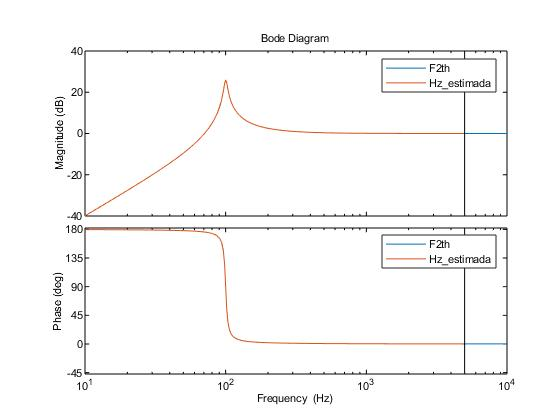
\includegraphics[scale=0.5]{highpassdiscrete}
  \caption{Respuesta en frecuencia del filtro paso alto de segundo orden}
  \label{fig:highpassdiscrete}
\end{figure}

\subsubsection{Implementación}
Al método software que se encarga de ejecutar este filtrado , se le deberán pasar los siguientes parámetros:
\begin{enumerate}
\item Frecuencia de muestro 
\item Frecuencia de corte
\item Factor de calidad
\end{enumerate}
Con estos parámetros el método software se encargará de extraer los coeficientes como se ha visto en los puntos anteriores y, realizar el filtrado de la muestra de entrada.


\section{Filtros de orden superior}
\subsection{Descripción}
Las formas directas no resultan útiles cuando el orden de la función a realizar es elevado, ya que su sensibilidad con respecto a la cuantificación de los coeficientes aumenta enormemente con el grado de la función. Para evitar este problema se suelen descomponer las funciones del sistema como suma o producto de funciones de primer y segundo orden, las cuales podrán realizarse según algunas de las formas ya vistas en el documento.

La forma de realizar el filtro es en cascada, y sigue los siguiente pasos:
\begin{enumerate}
\item Factorizamos los polinomios del numerador y denominador, agrupando las raíces conjugadas para que no aparezcan coeficientes complejos.
\begin{equation}
H(z)=A\frac{\prod_{k=1}^{M_{1}}(1-g_kz^{-1})\prod_{k=1}^{M_{2}}(1-h_kz^{-1})(1-h_k^*z^{-1})}{\prod_{k=1}^{N_{1}}(1-c_kz^{-1})\prod_{k=1}^{N_{2}}(1-d_kz^{-1})(1-d_k^*z^{-1})}
\end{equation}

\item  Expresamos H(z) como producto de funciones de segundo orden, donde N es el menor
entero mayor o igual que N/2. 

\begin{equation}
H(z)=\prod_{k=1}^{N_s}\frac{b_{0k}+b_{1k}z^{-1}+b_{2k}z^{-2}}{1-a_{1k}z^{-1}-a_{2k}z^{-2}}
\end{equation}

\item  Se realizan las funciones  de segundo orden en la forma directa II y se conectan en cascada como indica la figura.
\begin{figure}[H]
  \centering
	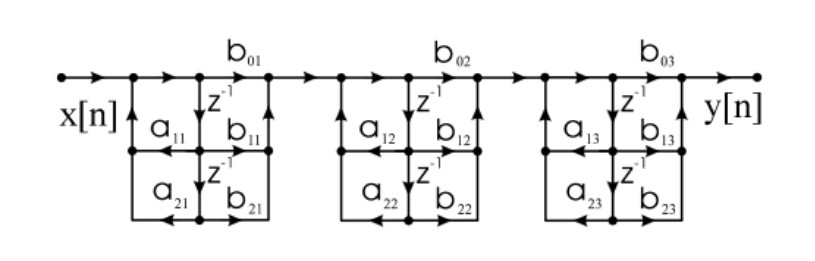
\includegraphics[scale=0.5]{forma_directa_II}
  \caption{Ejemplo de tres secciones de segundo orden en forma directa II}
  \label{fig:forma_directa_II}
\end{figure}
\end{enumerate}

\subsection{Implementación}
Al método software que se encarga de ejecutar este filtrado , se le deberán pasar los coeficientes del filtro en dos arrays, uno que identifica los coeficientes $a_{k}$ de las secciones de segundo orden, y otro con los coeficientes $b_k$. Él método por si mismo se encarga de ejecutar a partir de estos coeficientes una estructura en cascada como la vista en la figura \ref{fig:forma_directa_II}.

\subsection{Ejemplo en Matlab de la obtención de secciones de segundo orden}
En el siguiente script se puede ver un ejemplo de un filtro Butterworth con dos secciones de segundo orden. 
\lstset{language=Matlab,%
    basicstyle=\scriptsize,
    breaklines=true,%
    morekeywords={matlab2tikz},
    keywordstyle=\color{blue},%
    morekeywords=[2]{1}, keywordstyle=[2]{\color{black}},
    identifierstyle=\color{black},%
    stringstyle=\color{mylilas},
    commentstyle=\color{mygreen},%
    showstringspaces=false,%without this there will be a symbol in the places where there is a space
%    numbers=left,%
    numberstyle={\tiny \color{black}},% size of the numbers
    numbersep=9pt, % this defines how far the numbers are from the text
    emph=[1]{for,end,break},emphstyle=[1]\color{red}, %some words to emphasise
    %emph=[2]{word1,word2}, emphstyle=[2]{style},    
}
\lstinputlisting{butterworth.m}

\end{document}
